\documentclass[11pt,a4paper]{article}

\usepackage[utf8]{inputenc}
\usepackage[T1]{fontenc}
\usepackage{lmodern}
\usepackage[a4paper,margin=2.2cm]{geometry}
\usepackage{graphicx}
\usepackage{booktabs}
\usepackage{tabularx}
\usepackage{array}
\usepackage{amsmath}
\usepackage{amssymb}
\usepackage{siunitx}
\usepackage{float}
\usepackage{enumitem}
\usepackage{xcolor}
\usepackage{hyperref}
\usepackage{caption}
\usepackage{listings}
\usepackage{fancyhdr}
\usepackage{eso-pic}
\usepackage{transparent}

\hypersetup{hidelinks}
\setlength{\parskip}{0.5em}
\setlength{\parindent}{0pt}
\captionsetup{font=small,labelfont=bf}
\sisetup{round-mode=places,round-precision=2}

\definecolor{accent}{HTML}{8B1E3F}
\definecolor{lightgray}{HTML}{F5F5F5}

\pagestyle{fancy}
\fancyhf{}
\fancyhead[L]{IoT Challenge \#1 Report}
\fancyhead[R]{\thepage}
\renewcommand{\headrulewidth}{0.3pt}
\setlength{\headheight}{14pt}

\lstdefinestyle{codestyle}{
  basicstyle=\ttfamily\footnotesize,
  backgroundcolor=\color{lightgray},
  frame=single,
  breaklines=true,
  columns=fullflexible,
  showstringspaces=false,
  language=C++,
  keywordstyle=\color{blue},
  commentstyle=\color{green!50!black},
  stringstyle=\color{red}
}
\lstset{style=codestyle}

\begin{document}

\begin{titlepage}
\begin{figure}[H]
\centering

\includegraphics[width=0.88\textwidth]{figures/Picture4.png}
\end{figure}
\centering
%{\Large Politecnico di Milano\par}
\vspace{0.8cm}
{\huge\bfseries IoT Challenge \#1 Report\par}
\vspace{0.25cm}
{\Large Wokwi Motion Sensor Node with ESP-NOW Communication and Energy Estimation\par}
\vspace{0.5cm}
{\large Course material: Wokwi and Power Consumption\par}
\vspace{1.2cm}
\begin{tabular}{>{\bfseries}l l}
Student 1: & Mobin Khatib (11114435) \\
Student 2: & Ali Edareh Heidarabadi (110360280)\\
\end{tabular}
\vfill
\vfill
{\large March 2026\par}



\end{titlepage}
\AddToShipoutPictureBG*{
\AtPageCenter{
\transparent{0.15}
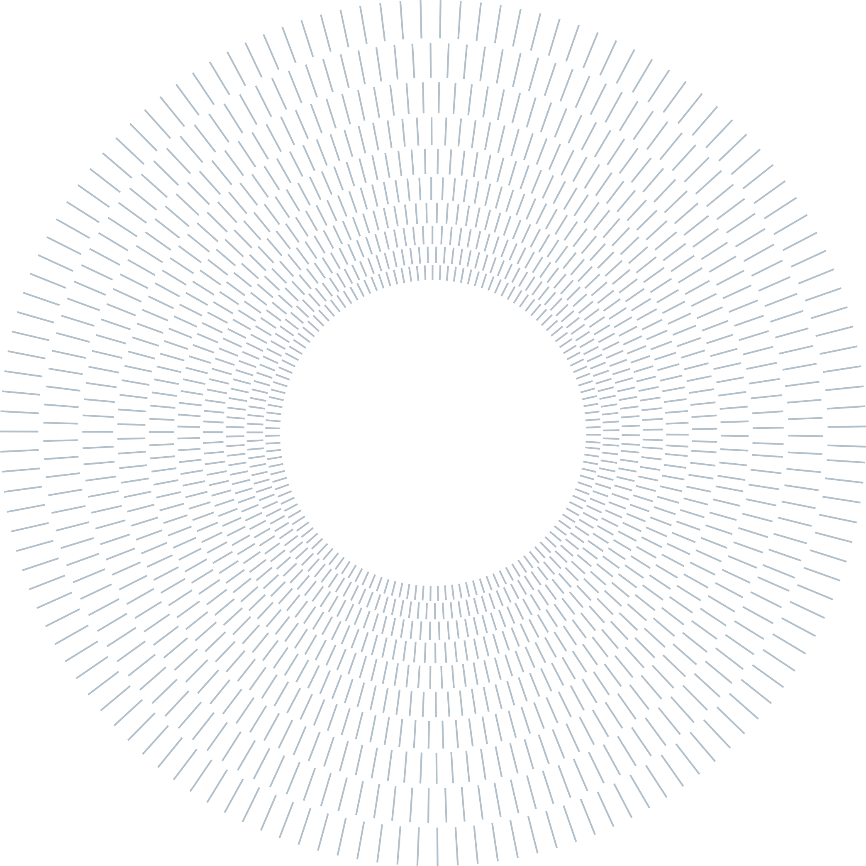
\includegraphics[width=0.9\paperwidth]{figures/Picture3.png}
}
}
\section*{Executive summary}
This report documents an ESP32-based smart-home motion sensor implemented in Wokwi. The node reads a PIR motion sensor and an LDR, formats the result as a single ESP-NOW message, and then enters timer-driven deep sleep. The energy model combines power levels extracted from the laboratory CSV traces with timing values derived from the Wokwi implementation. For reporting clarity, the awake interval is decomposed into five physical states --- Boot, Sensor Reading, Wi-Fi On / ESP-NOW Init, Transmission, and Post-TX Idle --- plus one derived summary row, Total Awake Time. The baseline case uses the default transmission mode visible in the sender trace, corresponding to \SI{19.5}{dBm}; the improvement study replaces only that transmission state with the \SI{2}{dBm} mode. The results show that the dominant contributors are Deep Sleep and Wi-Fi initialization, while lowering TX power has a measurable but small impact on total cycle energy.

\section{System specification and implementation}
\subsection{Objective}
The sensor node must detect motion, estimate ambient light, and send a single string to a sink node using one of the following formats:
\[
\texttt{MOTION\_DETECTED-LUMINOSITY:ZZZ}
\qquad \text{or} \qquad
\texttt{MOTION\_NOT\_DETECTED-LUMINOSITY:ZZZ}.
\]
The sink node is assumed reachable and therefore was not implemented inside the emulator.

With leader code \texttt{11114435}, the sleep interval is
\[
X = \frac{(35 \bmod 50) + 5}{10} = \SI{4.0}{s}.
\]
The battery energy used in the lifetime estimate is
\[
Y = (4435 \bmod 5000) + 15000 = \SI{19435}{J}.
\]

The firmware sequence is: boot and initialize Wi-Fi/ESP-NOW, read the PIR and LDR, convert the LDR voltage-divider measurement into an approximate lux value, assemble the payload string, transmit it, and return to deep sleep.

\begin{figure}[H]
\centering
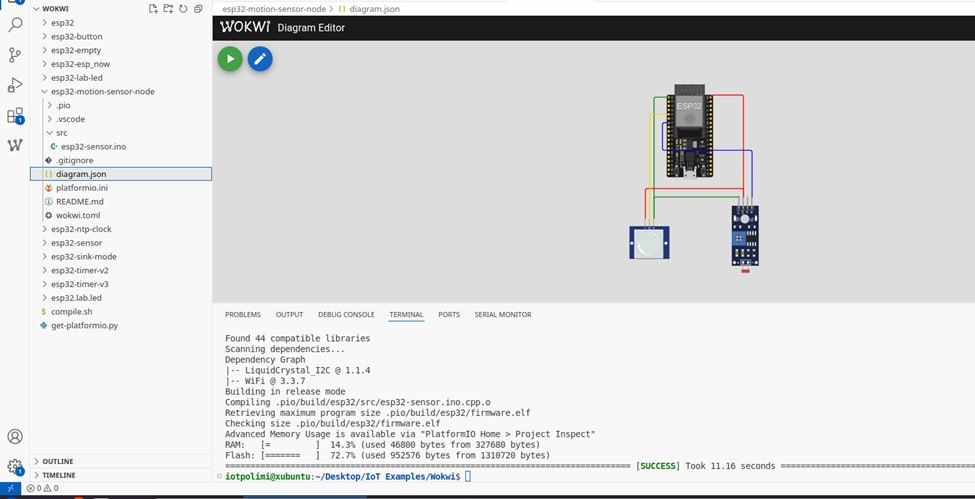
\includegraphics[width=0.88\textwidth]{figures/wokwi_setup.png}
\caption{Wokwi implementation used for the report: ESP32 connected to the PIR sensor and the LDR module.}
\end{figure}

\subsection{Firmware logic}
The PIR sensor is read from \texttt{GPIO34} as a digital input. The photoresistor module is read from \texttt{GPIO32}, which belongs to ADC1 and therefore avoids the ADC2/Wi-Fi conflicts typical of the ESP32.

The ADC reading is converted to voltage with a \SI{3.3}{V} reference, translated into resistance using a \SI{2}{k\ohm} voltage-divider model, and then mapped to an approximate light level using the empirical Wokwi photoresistor model:
\[
V = \frac{\texttt{analogValue}}{4095} \cdot 3.3,
\qquad
R_{\mathrm{LDR}} = 2000\,\frac{V}{3.3 - V},
\]
\[
\text{light} = \left(\frac{RL_{10}\cdot 1000\cdot 10^{\gamma}}{R_{\mathrm{LDR}}}\right)^{1/\gamma},
\qquad RL_{10}=50,\; \gamma=0.7.
\]
This is not a calibrated lux meter, but it is sufficient for relative bright/dark estimation in the smart-home use case.

ESP-NOW is initialized in station mode and the broadcast address \texttt{FF:FF:FF:FF:FF:FF} is registered as the peer. The loop then sends the motion/luminosity string and immediately enters deep sleep.

\subsection{Key implementation excerpt}
The following code implements the sensing, transmission, and deep sleep logic as described.

\subsubsection*{Library Imports and Hardware Definitions}

\begin{lstlisting}
#define PIR_PIN 34 
#define LDR_PIN 32 

// Destination MAC address (Broadcast as per spec)
uint8_t broadcastAddress[] = {0xFF,0xFF,0xFF,0xFF,0xFF,0xFF};
\end{lstlisting}

This section imports the required libraries and defines hardware connections.

\begin{itemize}
\item WiFi.h enables WiFi features on the ESP32.
\item esp-now.h enables the ESP-NOW protocol for low-power wireless communication between ESP devices.
\end{itemize}

The <broadcastAddress> is set to FF:FF:FF:FF:FF:FF, which means the ESP32 will broadcast messages to all nearby ESP-NOW devices instead of sending to a specific device.

\subsubsection*{System Initialization}

\begin{lstlisting}
void setup() {

  Serial.begin(115200);

  // Set PIR sensor pin as input
  pinMode(PIR_PIN, INPUT);

  // Initialize WiFi in Station mode for ESP-NOW
  WiFi.mode(WIFI_STA);

  if (esp_now_init() != ESP_OK) {
    Serial.println("Error initializing ESP-NOW");
    return;
  }

  // Define and register the peer information
  esp_now_peer_info_t peerInfo = {};

  memcpy(peerInfo.peer_addr, broadcastAddress, 6);
  peerInfo.channel = 0;
  peerInfo.encrypt = false;

  esp_now_add_peer(&peerInfo);
}
\end{lstlisting}

This section initializes the system and configures wireless communication.

\begin{itemize}
\item Serial communication is started for debugging.
\item The PIR pin is configured as an input.
\item The ESP32 is set to station mode, which is required for ESP-NOW operation.
\end{itemize}

Then the ESP-NOW protocol is initialized and a broadcast peer is added so the device can transmit data to other nodes.

\textbf{Note:}

In ESP-NOW communication, a peer device must be registered before sending data.

In this implementation, a broadcast peer is added using the MAC address FF:FF:FF:FF:FF:FF. This allows the ESP32 node to transmit messages to any nearby receiver without specifying a specific device. This broadcast functionality is exclusive to the all-ones MAC address (FF:FF:FF:FF:FF:FF), enabling the ESP32 to transmit data to any listening node in its vicinity without the need for individual device pairing.

\textbf{Note:}
A 10ms guard delay for sensor stabilization was intentionally omitted to maintain strict consistency with the physical laboratory traces. By excluding this delay, the energy estimation remains more realistic, as it directly aligns with the hardware behavior captured in the provided CSV datasets.
\subsubsection*{Sensor Reading}

\begin{lstlisting}
void loop() {

  //start timing sensing sensor
  unsigned long t_start_sensing = micros();

  // Read digital signal from PIR and analog value from LDR
  int motion = digitalRead(PIR_PIN);
  int analogValue = analogRead(LDR_PIN);
\end{lstlisting}

This section reads the data from the sensors.

The PIR motion sensor detects whether motion is present.

The LDR sensor provides an analog value corresponding to the ambient light level.

The sensing start time is also recorded to measure the sensing duration.

\subsubsection*{LDR Lux Conversion}

\begin{lstlisting}
  // Parameters of the LDR model
  const float GAMMA = 0.7;
  const float RL10 = 50;
  // Convert ADC value to voltage (ESP32: 0–4095, 3.3V reference)
  float voltage = analogValue / 4095.0 * 3.3;
  // Calculate LDR resistance using the voltage divider formula (2kΩ resistor)
  float resistance = 2000 * voltage / (3.3 - voltage);
  // Convert resistance to light intensity (lux)
  float light = pow(RL10 * 1000 * pow(10, GAMMA) / resistance, (1 / GAMMA));
  // long duration sensing
  unsigned long duration_sensing = micros() - t_start_sensing;
  // timing sending part
  unsigned long t_start_tx = micros();
\end{lstlisting}

Using the voltage divider equation, the voltage is then used to compute the resistance of the LDR.

However, illuminance is required in lux, not resistance. An empirical relationship between LDR resistance and light intensity is therefore used.

$RL_{10}$ represents the LDR resistance at $10\,\text{lux}$, and $\gamma$ describes how the resistance changes with light.

Using these parameters, the resistance is converted into an approximate lux value.

\[
\text{calculated lux} \approx 10 \times \text{actual lux}
\]

This happens because the constants ($RL_{10}$ and $\gamma$) in the photoresistor model used in Wokwi are approximate.

The behavior is still correct because:

\begin{itemize}
\item darker → smaller number
\item brighter → larger number
\item the relationship is proportional
\end{itemize}

\subsubsection*{Transmission and Deep Sleep}

\begin{lstlisting}
String message;

if(motion == HIGH){
  message = "MOTION_DETECTED-LUMINOSITY:" + String(light);
}
else{
  message = "MOTION_NOT_DETECTED-LUMINOSITY:" + String(light);
}

esp_now_send(broadcastAddress, (uint8_t*)message.c_str(), message.length());
// End timing and printing
unsigned long t_end_tx = micros();
unsigned long duration_tx = t_end_tx - t_start_tx;

// Print time needed for energy estimation
Serial.print("Sensing Time (us): "); Serial.println(duration_sensing);
Serial.print("TX Time (us): "); Serial.println(duration_tx);
Serial.println(message);
Serial.println("Going to deep sleep...");

esp_sleep_enable_timer_wakeup(4 * 1000000);
esp_deep_sleep_start();
\end{lstlisting}

This section creates the message containing the motion status and the measured light intensity.

If motion is detected, the message includes \texttt{MOTION\_DETECTED}, otherwise \texttt{MOTION\_NOT\_DETECTED}. The measured light value (lux) is appended to the message.

Before sending the message, the transmission start time is recorded using \texttt{micros()}. The message is then transmitted using ESP-NOW.

After the transmission, the end time is recorded again using \texttt{micros()}. The difference between the start and end times gives the transmission duration.

Finally, the ESP32 enters Deep Sleep Mode for $4$ seconds to reduce energy consumption before repeating the sensing cycle.
\subsection*{Important Implementation Notes}

\subsubsection*{Analog Pins on the ESP32}

The ESP32 has two groups of analog pins:

\begin{itemize}
\item ADC1 (32--39)
\item ADC2 (0, 2, 4, 12--15, 25--27)
\end{itemize}

Pins from ADC2 may conflict with WiFi features, including ESP-NOW. Therefore, it is recommended to use ADC1 pins for \texttt{analogRead()}.

In this project, the LDR sensor is connected to pin 32, which ensures reliable analog readings while WiFi communication is active.

\subsubsection*{PIR Sensor Delay in Simulation}

The PIR motion sensor usually has a default delay of about $5$ seconds, meaning the output remains HIGH for a short time after motion is detected.

In the Wokwi environment, this delay can be changed in the \texttt{diagram.json} file:

\begin{verbatim}
{ "type": "wokwi-pir-motion-sensor", "id": "pir1",
  "top": 182.4, "left": -83.62, "rotate": 180,
  "attrs": { "delay": "2" } }
\end{verbatim}

This example sets the PIR sensor delay to $2$ seconds in the simulation.

\section{Measurement methodology}
\subsection{Measurement sources}
Two different information streams are combined:
\begin{itemize}[leftmargin=1.5em]
\item the power traces from \texttt{deep\_sleep.csv}, \texttt{sensor-read.csv}, and \texttt{sender.csv}, which provide average power levels for each modeled state;
\item direct timing measurements from Wokwi, where \texttt{micros()} is used around the sensing and transmission operations.
\end{itemize}
Boot time, Wi-Fi initialization time, and Post-TX idle time are modeled from the plateaus in \texttt{deep\_sleep.csv}. Deep sleep is fixed by the challenge requirement at \SI{4.0}{s}.

\subsection{State decomposition used in the report}
For reporting clarity, the awake interval is decomposed into five physical states and one derived summary row:
\begin{enumerate}[leftmargin=1.5em]
\item Boot
\item Sensor Reading
\item Wi-Fi On / ESP-NOW Init
\item Transmission
\item Post-TX Idle
\item Total Awake Time (derived)
\end{enumerate}
The last row is not a physical state; it is included only to summarize the full awake interval before deep sleep.

\begin{table}[H]
\centering
\caption{Six-row awake decomposition used in the baseline report. The last row is a derived summary row, not a physical state.}
\begin{tabular}{lccc}
\toprule
Awake phase / row & Source file & Average power (mW) & Duration (s) \\
\midrule
Boot & \texttt{deep\_sleep.csv} & 251.82 & 0.100000 \\
Sensor Reading & \texttt{sensor-read.csv} & 351.09 & 0.000892 \\
Wi-Fi On / ESP-NOW Init & \texttt{deep\_sleep.csv} & 633.23 & 0.190000 \\
Transmission (19.5 dBm) & \texttt{sender.csv} & 668.48 & 0.001039 \\
Post-TX Idle & \texttt{deep\_sleep.csv} & 251.82 & 0.050000 \\
\midrule
Total Awake Time (derived) & Derived & 465.28 & 0.341932 \\
\bottomrule
\end{tabular}
\end{table}

\subsection{Timing values and extraction rules}
The timing values used in the energy model are summarized in Table~\ref{tab:timing}. The boot and Wi-Fi/Post-TX durations are obtained from the deep-sleep reference trace, while sensor and transmission durations are measured directly in firmware.

\begin{table}[H]
\centering
\caption{Timing parameters used in the energy model.}
\label{tab:timing}
\begin{tabular}{p{3.2cm}p{3.0cm}p{6.4cm}c}
\toprule
State & Source & Extraction rule & Duration (s) \\
\midrule
Boot & \texttt{deep\_sleep.csv} & First wake-up to first 251 mW plateau & 0.100000 \\
Sensor Reading & Wokwi Serial Monitor & 19-run average of \texttt{micros()}-based measurement & 0.000892 \\
Wi-Fi On / ESP-NOW Init & \texttt{deep\_sleep.csv} & Duration of the 633 mW plateau & 0.190000 \\
Transmission & Wokwi Serial Monitor & 19-run average of \texttt{micros()}-based measurement & 0.001039 \\
Post-TX Idle & \texttt{deep\_sleep.csv} & Final 251 mW plateau before the sleep floor & 0.050000 \\
Deep Sleep & Firmware requirement & $X$ derived from team leader code & 4.000 \\
\bottomrule
\end{tabular}
\end{table}

The 19 repeated Wokwi measurements give an average sensing time of \SI{892.37}{\micro s} and an average transmission time of \SI{1039.47}{\micro s}. The minimum, maximum, and average values are shown below.

\begin{table}[H]
\centering
\caption{Summary statistics of the 19 Wokwi timing measurements.}
\begin{tabular}{lcc}
\toprule
Statistic & Sensing Time (\si{\micro s}) & Transmission Time (\si{\micro s}) \\
\midrule
Count & 19 & 19 \\
Minimum & 815 & 963 \\
Maximum & 1053 & 1092 \\
Average & 892.37 & 1039.47 \\
\bottomrule
\end{tabular}
\end{table}

\begin{figure}[H]
\centering
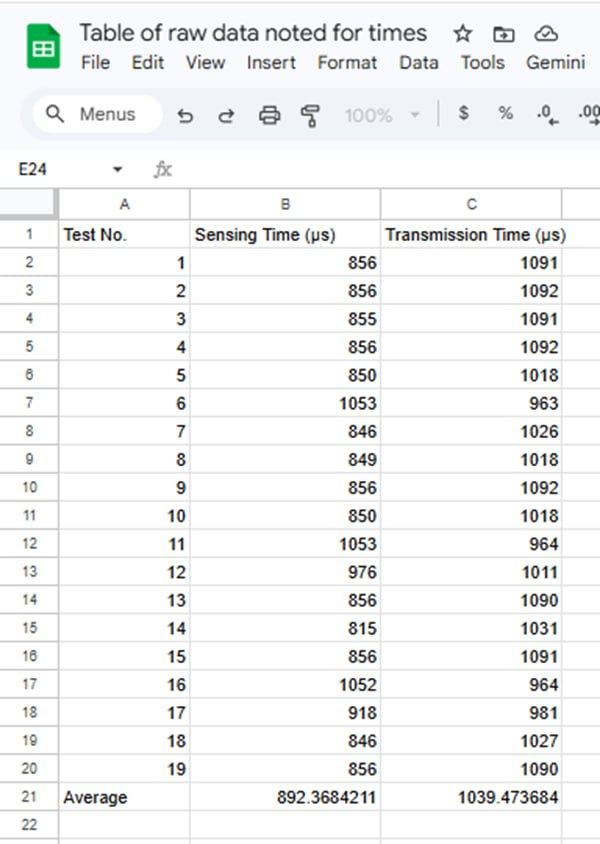
\includegraphics[width=0.75\textwidth]{figures/timing_raw_table.png}
\caption{Raw Wokwi timing table used to compute the average sensing and transmission durations.}
\end{figure}

\subsection{Threshold reasoning for power extraction}
Average power values were not computed as whole-file means. Instead, threshold windows were used to isolate the relevant plateau or spike associated with each state.

\begin{table}[H]
\centering
\caption{Threshold windows used to isolate each power state from the CSV traces.}
\begin{tabular}{p{4.0cm}p{2.7cm}p{7.0cm}}
\toprule
State & Threshold & Rationale \\
\midrule
Deep Sleep & $< \SI{100}{mW}$ & Isolates the stable floor and excludes wake-up transitions. \\
Boot / Post-TX Idle & \SIrange{245}{258}{mW} & Targets the stable middle plateau with CPU on and Wi-Fi off. \\
Wi-Fi On / ESP-NOW Init & $> \SI{600}{mW}$ & Captures the radio-on/calibration plateau before payload transmission. \\
Sensor Reading & $> \SI{340}{mW}$ & Separates sensor activity from the lower idle plateau in the sensor trace. \\
Transmission (baseline) & $\geq \SI{650}{mW}$ & Captures ESP-NOW TX spikes at the default \SI{19.5}{dBm} setting. \\
Transmission (improved) & \SIrange{615}{625}{mW} & Captures the lower-power \SI{2}{dBm} TX pulses in the sender trace. \\
\bottomrule
\end{tabular}
\end{table}

\begin{figure}[H]
\centering
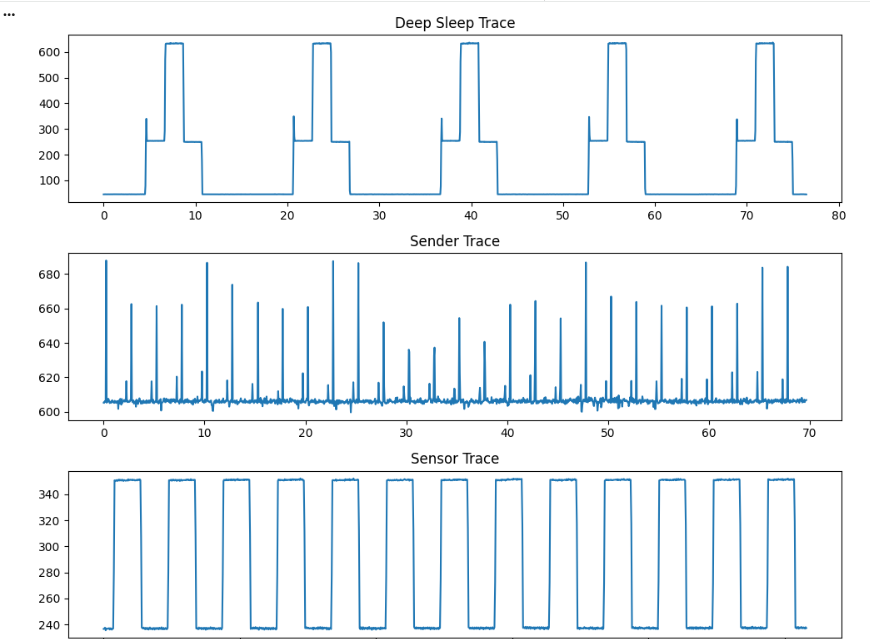
\includegraphics[width=0.90\textwidth]{figures/power_traces_overview.png}
\caption{Overview of the three provided power traces. Thresholds are applied to isolate the relevant plateaus and transmission spikes.}
\end{figure}

\subsection*{Power Threshold Reasoning}

\begin{itemize}

\item \textbf{Deep Sleep (< 100 mW):} This isolates the ``floor'' power consumption. 
It ensures that only the passive state is averaged, excluding any noise or transitions 
from the CPU waking up.

\item \textbf{Boot / Post-TX Idle (245 to 258 mW):} This specific window targets the 
stable ``middle plateau''. It represents the ESP32 being active (CPU on) but without 
the high-draw Wi-Fi radio active.

\item \textbf{Wi-Fi Init (> 600 mW):} The Wi-Fi radio calibration causes a massive 
jump. Using a high threshold ensures we capture the peak power required to 
``start'' the radio before transmission.

\item \textbf{Sensor Reading (> 340 mW):} Sensing requires more power than idling 
but less than Wi-Fi. This threshold separates the I2C/analog sensor activity 
from the background noise of the microcontroller.
The sensor-read trace is utilized as the generic reference for sensing activity, as requested by the assignment specifications, ensuring the energy model remains consistent with the provided laboratory benchmark
\item \textbf{Transmission (>= 650 mW):} ESP-NOW transmission at maximum power 
(19.5 dBm) creates the highest current spikes. This value specifically captures 
the ``TX'' pulses, ignoring the lower-power ``listen'' or ``idle'' states.

\end{itemize}

\subsection*{Timing Precision Reasoning}

\[
892.37 \times 10^{-6} \; \text{s (Sensor)} 
\quad \text{and} \quad 
1039.47 \times 10^{-6} \; \text{s (TX)}
\]

These aren't guesses; they are modeled durations using \texttt{micros()} in firmware. 
Since these events happen in microseconds, using a rounded number such as $0.001$ s 
would cause a significant error in the final energy ($E$) calculation.
\section{Power and energy estimation}
\subsection{Average power per state}
Applying the threshold windows to the traces yields the average power values in Table~\ref{tab:power}. The baseline transmission state corresponds to the default sender mode at \SI{19.5}{dBm}. For comparison, the \SI{2}{dBm} transmission average is also reported for the improvement study.

\textbf{Note}: 

The Boot and Post-TX Idle phases exhibit identical power signatures (approx. $251$ mW) because in both states, the ESP32 CPU is active at full clock speed while the energy-intensive Wi-Fi radio remains powered down or in a low-power wait state.
\begin{table}[H]
\centering
\caption{Average power values extracted from the provided laboratory traces.}
\label{tab:power}
\begin{tabular}{lcc}
\toprule
State & Source & Average power (mW) \\
\midrule
Boot & \texttt{deep\_sleep.csv} & 251.82 \\
Sensor Reading & \texttt{sensor-read.csv} & 351.09 \\
Wi-Fi On / ESP-NOW Init & \texttt{deep\_sleep.csv} & 633.23 \\
Transmission (19.5 dBm) & \texttt{sender.csv} & 668.48 \\
Transmission (2 dBm) & \texttt{sender.csv} & 618.91 \\
Post-TX Idle & \texttt{deep\_sleep.csv} & 251.82 \\
Deep Sleep & \texttt{deep\_sleep.csv} & 45.78 \\
\bottomrule
\end{tabular}
\end{table}

\subsection{Baseline cycle energy}
The baseline cycle uses the five physical awake states, the default transmission plateau at \SI{19.5}{dBm}, and a deep-sleep interval of \SI{4.0}{s}. Energy is computed for each state as
\[
E_i = P_i \times T_i.
\]

\begin{table}[H]
\centering
\caption{Baseline cycle-energy calculation with the default \SI{19.5}{dBm} transmission state.}
\begin{tabular}{lcccc}
\toprule
State & Power (mW) & Duration (s) & Energy (mJ) & Share (\%) \\
\midrule
Boot & 251.82 & 0.100000 & 25.182 & 7.359 \\
Sensor Reading & 351.09 & 0.000892 & 0.313306 & 0.091556 \\
Wi-Fi On / ESP-NOW Init & 633.23 & 0.190000 & 120.31 & 35.159 \\
Transmission (19.5 dBm) & 668.48 & 0.001039 & 0.694868 & 0.203059 \\
Post-TX Idle & 251.82 & 0.050000 & 12.591 & 3.679 \\
Deep Sleep & 45.78 & 4.000 & 183.11 & 53.509 \\
\midrule
Total & --- & 4.342 & 342.20 & 100.00 \\
\bottomrule
\end{tabular}
\end{table}

\begin{figure}[H]
\centering
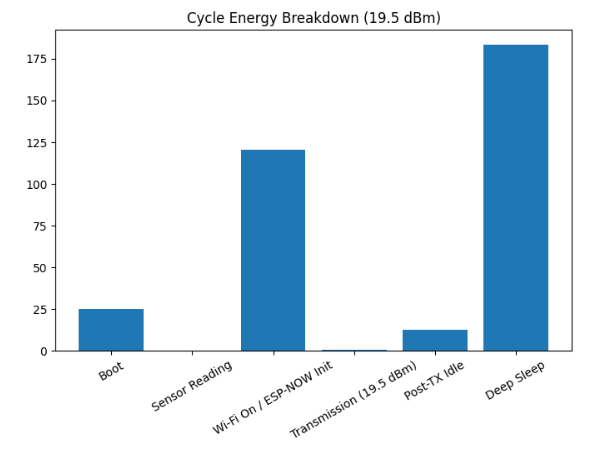
\includegraphics[width=0.82\textwidth]{figures/energy_breakdown_baseline.png}
\caption{Baseline energy contribution by state.}
\end{figure}

The baseline cycle energy is \SI{342.20}{mJ} over a cycle time of \SI{4.341932}{s}. Deep Sleep contributes 53.51\% of the energy, while Wi-Fi On / ESP-NOW Init contributes 35.16\%. The transmission state itself is below 1\% of the cycle total.

\subsection{Battery lifetime estimate}
Using \(Y = \SI{19435}{J}\), the baseline lifetime estimate is
\[
N_{\text{cycles}} = \frac{19435}{0.34220} \approx 56794,
\qquad
T_{\text{life}} = N_{\text{cycles}} \cdot 4.341932 \approx \SI{68.50}{h}.
\]
Therefore, under the laboratory power model used here, the node can operate for about \SI{68.50}{h} before the battery energy is exhausted.

\section{Discussion and improvements}
The six-row awake decomposition changes the interpretation of the system compared with the coarse three-phase model. Once the deep-sleep plateau is isolated correctly, the dominant contributors are Deep Sleep and Wi-Fi initialization rather than the transmission spikes themselves.

The measured deep-sleep power of about \SI{45.78}{mW} still includes the laboratory overhead of the measurement environment. In a production implementation powered without the USB bridge and with a low-leakage regulator, the true sleep floor would be much smaller.

\subsection{Analysis of System Optimization and Energy Constraints}

Based on the laboratory power traces and the detailed breakdown, it is evident that the opportunities for reducing energy consumption within a single operational cycle are strictly limited by hardware-defined plateaus.

\subsection{Inherent Constraints and Fixed States}
The energy model identifies several states that are essentially \textbf{fixed} due to hardware initialization requirements and environmental overhead:
\begin{itemize}
    \item \textbf{Boot and Post-TX Idle:} These durations ($0.1\text{ s}$ and $0.05\text{ s}$) are determined by the ESP32's internal wake-up and stabilization cycles .
    \item \textbf{Wi-Fi / ESP-NOW Initialization:} This is the most energy-intensive awake state, accounting for \textbf{35.16\%} of the total cycle energy ($120.31\text{ mJ}$). This calibration phase cannot be bypassed by firmware.
    \item \textbf{Deep Sleep:} Accounting for \textbf{53.51\%} of the total energy due to its long $4$-second duration .
\end{itemize}

\subsection{Synergy of Firmware and Hardware Optimization}
The only parameters subject to optimization are the \textbf{Sensor Reading}, \textbf{Transmission duration}, and \textbf{TX Power levels}. However, these states collectively represent less than \textbf{1\%} of the total energy share. 
By combining firmware optimization (reducing sensing and TX times) with hardware optimization (switching from $19.5\text{ dBm}$ to $2\text{ dBm}$), the cycle energy decreases from $\mathbf{342.20\text{ mJ}}$ to $\mathbf{341.41\text{ mJ}}$. The results of this cumulative optimization are summarized in Table \ref{tab:combined_opt}.
The parameters that can be optimized are limited to the \textbf{sensor reading time}, \textbf{transmission duration}, and \textbf{TX power levels}. However, these states together account for less than \textbf{1\%} of the total energy consumption.

With the improved firmware implementation (second version of the code), the measured timings are:

\begin{itemize}
    \item \textbf{Sensor reading time:} 333\,\si{\micro\second}
    \item \textbf{Transmission time:} 214\,\si{\micro\second}
\end{itemize}

These very short active durations confirm that the node spends the vast majority of its lifetime in low-power sleep states, and therefore firmware optimizations mainly affect a very small fraction of the total energy budget.
\begin{table}[h!]
\centering
\caption{Cumulative Effect of Single-Cycle Optimizations}
\label{tab:combined_opt}
\begin{tabular}{lccc}
\hline
\textbf{Operational State} & \textbf{Baseline (mJ)} & \textbf{Combined Optimized (mJ)} & \textbf{Energy Share (\%)} \\ \hline
Boot                       & 25.18                  & 25.18 (Fixed)                    & 7.359                      \\
Sensor Reading             & 0.31                   & \textbf{0.12}                    & 0.092                      \\
Wi-Fi / ESP-NOW Init       & 120.31                 & 120.31 (Fixed)                   & 35.159                     \\
Transmission               & 0.69                   & \textbf{0.09}                    & 0.203                      \\
Post-TX Idle               & 12.59                  & 12.59 (Fixed)                    & 3.679                      \\
Deep Sleep                 & 183.12                 & 183.12 (Fixed)                   & 53.509                     \\ \hline
\textbf{Total per Cycle}   & \textbf{342.20}        & \textbf{341.41}                  & \textbf{100.00}            \\ \hline
\end{tabular}
\end{table}

\subsection{Strategic Shift: Event-Driven Operation}
As demonstrated, single-cycle optimizations yield negligible returns because the dominant energy consumers (Wi-Fi Init and Sleep) remain unchanged. To achieve meaningful energy savings, the system must transition from a periodic model to an \textbf{Event-Driven} model. By reducing the transmission frequency (e.g., to $100$ events per $24$-hour window), the average power consumption drops significantly, as the node avoids the repeated cost of radio startup when no motion is detected.
\begin{table}[H]
\centering
\caption{Quantitative comparison of baseline and cumulative optimized cycles.}
\label{tab:final_comparison}
\begin{tabular}{lcc}
\toprule
Scenario & Cycle Energy (mJ) & Estimated Lifetime (h) \\
\midrule
Baseline (19.5 dBm) & 342.20 & 68.50 \\
Optimized Firmware (19.5 dBm) & 341.46 & 68.65 \\
Combined Optimized (2 dBm) & 341.41 & 68.66 \\
\midrule
\textbf{Total Absolute Improvement} & \textbf{0.79} & \textbf{0.16} \\
\bottomrule
\end{tabular}
\end{table}

\subsection{Additional improvements suggested by the data}

Based on the measured energy distribution, the most effective optimizations focus on reducing unnecessary wake-ups, minimizing radio active time, and avoiding redundant transmissions.

\textbf{1. Event-driven wake-up with PIR interrupt.}

The periodic timer wake-up was removed and the ESP32 now enters deep sleep with an external wake-up source on the PIR output using \texttt{esp\_sleep\_enable\_ext0\_wakeup(GPIO\_NUM\_34, 1)}. In this architecture, the node sleeps indefinitely and wakes only when motion is detected. This removes redundant wake-up, radio-initialization, and transmission cycles that previously occurred even when the environment had not changed.

Because \texttt{EXT0} wake-up is level-triggered, the firmware waits for the PIR output to return LOW before arming sleep again, preventing immediate re-wake loops. The deep-sleep and ESP-NOW control flow follows the capabilities provided by the Espressif software stack~[1].

\textbf{2. Communication energy optimization.}

The radio-active interval is reduced by two complementary techniques. First, the transmission path no longer depends on a fixed post-send delay. Instead, the ESP-NOW send callback is registered and used to detect when the transmission has actually completed. This allows the node to return to deep sleep immediately after the packet has been delivered by the protocol layer~[1].

Second, the Wi-Fi transmission power is reduced to \SI{2}{dBm} and the transmitted message is compressed from a long ASCII string such as \texttt{MOTION\_NOT\_DETECTED-LUMINOSITY:3094} into a compact 4-byte binary packet. The packet contains one byte for the motion flag, two bytes for luminosity, and one byte of state flags. This compression shortens airtime and simplifies parsing at the receiver, while the lower TX power reduces the RF energy per packet.

\textbf{3. Transmission only when the reported state changes.}

The optimized firmware stores the last transmitted motion/light state in retained memory across deep sleep and compares it with the newly measured state after each wake-up. If the state is unchanged, the ESP32 skips ESP-NOW transmission and returns directly to deep sleep, avoiding the radio cost.

This mechanism prevents repeated reports caused by multiple PIR triggers while the environmental condition remains unchanged. In the current PIR-triggered architecture, this logic effectively suppresses redundant ``motion detected'' messages, although a ``no motion'' transition cannot be reported proactively because the node wakes only on PIR activity.


\subsection{Evidence required after re-implementation}
The proposed optimizations must be supported by quantitative evidence. Because the optimized node is no longer periodic, the baseline fixed-cycle model cannot be compared directly to the new firmware using only one cycle number. A fair comparison should use the same observation window and the same environmental activity pattern for both systems. In the finalized comparison below, the observation window is \SI{24}{h}. Over that interval, the baseline periodic design performs 19,899 timer-driven wake/report cycles, while the optimized event-driven design is evaluated under a workload of 100 PIR-triggered report-worthy events.

For the optimized design, the key quantities to recompute are the total energy in the chosen observation window, the average power over that window, and the corresponding battery lifetime:
\[
P_{\mathrm{avg,opt}} = \frac{E_{\mathrm{win,opt}}}{T_{\mathrm{win}}},
\qquad
T_{\mathrm{life,opt}} = \frac{Y}{P_{\mathrm{avg,opt}}}.
\]
This normalization makes the comparison meaningful even though the optimized firmware no longer wakes up every \SI{4.0}{s}.

\begin{figure}[H]
\centering
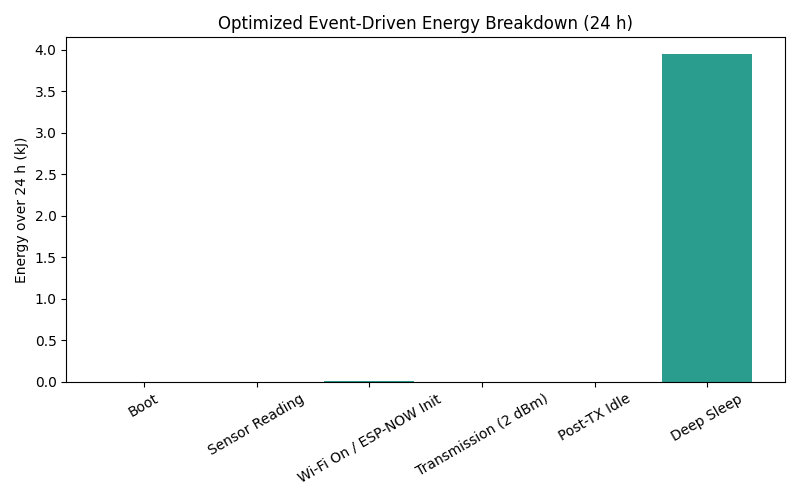
\includegraphics[width=0.82\textwidth]{figures/energy_breakdown_optimized_24h.png}
\caption{Recomputed energy breakdown of the optimized event-driven implementation over a \SI{24}{h} observation window.}
\label{fig:energy-optimized}
\end{figure}

\begin{figure}[H]
\centering
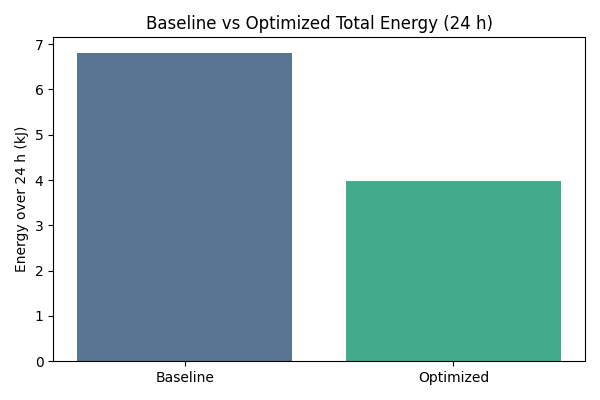
\includegraphics[width=0.72\textwidth]{figures/energy_compare_24h.png}
\caption{Direct comparison between the original periodic design and the optimized event-driven design over a \SI{24}{h} observation window.}
\label{fig:energy-compare}
\end{figure}

\begin{table}[H]
\centering
\caption{Quantitative comparison between the baseline periodic design and the optimized event-driven design over a \SI{24}{h} observation window.}
\label{tab:improved-comparison}
\begin{tabular}{p{5.4cm}ccc}
\toprule
Metric & Baseline & Optimized & Relative change \\
\midrule
Observation window & 24 h & 24 h & --- \\
Triggering / report events in window & 19,899 & 100 & $-99.50\%$ \\
Total energy in window & 6.81 kJ (1.89 Wh) & 3.97 kJ (1.10 Wh) & $-41.70\%$ \\
Average power in window & 78.81 mW & 45.95 mW & $-41.70\%$ \\
Wi-Fi / ESP-NOW activations & 19,899 & 100 & $-99.50\%$ \\
Estimated lifetime & $L_{\mathrm{base}}$ & $1.72\,L_{\mathrm{base}}$ & $+71.53\%$ \\
\bottomrule
\end{tabular}
\end{table}

Table~\ref{tab:improved-comparison} shows that the strongest effect of the redesign is not a small reduction in the energy of one transmission, but a large reduction in how many times the ESP32 has to wake up and initialize the radio. Over the \SI{24}{h} window, Wi-Fi / ESP-NOW activations drop from 19,899 to 100, which leads to a 41.70\% reduction in total energy and average power. The energy reduction is smaller than the activation reduction because the node still spends energy in deep sleep and because every remaining event still pays a nonzero boot and communication cost. The row labeled ``Triggering / report events'' should be interpreted as periodic timer wake/report cycles in the baseline case and PIR-triggered report-worthy events in the optimized case. Even so, the practical impact is substantial: the estimated lifetime increases to $1.72\,L_{\mathrm{base}}$, corresponding to a 71.53\% improvement.

\subsection{How the new plots should be interpreted}
Figure~\ref{fig:energy-optimized} should be read as the energy breakdown of the \emph{optimized} node over the same \SI{24}{h} observation window used in Table~\ref{tab:improved-comparison}. The key point is that the ESP32 no longer wakes up periodically just to send repeated information. Instead, it stays in deep sleep and wakes only when the PIR sensor triggers a relevant event. As a result, the main saving does not come from making one packet much cheaper, but from avoiding thousands of unnecessary wake-up and Wi-Fi / ESP-NOW initialization phases.

Figure~\ref{fig:energy-compare} should therefore be interpreted mainly as a comparison of \emph{how often} the full sensing-and-communication sequence is executed. In the baseline design, this sequence is repeated 19,899 times in \SI{24}{h}; in the optimized design, it happens only 100 times. That is why the total energy drops from \SI{6.81}{kJ} to \SI{3.97}{kJ}, even though each remaining transmission still has a nonzero boot and radio cost.

This is also why TX power reduction and compact packets are secondary improvements. They still reduce the energy of each report, but the dominant gain comes from the architectural change: removing unnecessary periodic wake-ups and repeated radio activation.
\subsection{Limitations and future work}
Under the optimized architecture, the lifetime is no longer determined by a single fixed cycle length, but by stochastic events such as motion arrivals, PIR hold times, and the number of packet transmissions over time. One natural follow-up is a Monte Carlo uncertainty analysis: one can sample motion-event patterns and communication outcomes repeatedly, compute the resulting energy usage over long horizons, and obtain a distribution of battery lifetime rather than a single deterministic number~[3]. This would make the robustness of the optimized design easier to evaluate under realistic usage variability.

\appendix
\section{Note: Raw Timing Averages}
The 19 manual timing samples extracted from the Wokwi serial monitor give the following averages used in the energy model:
\[
t_{\mathrm{sens}} = \SI{892.37}{\micro s}, \qquad t_{\mathrm{tx}} = \SI{1039.47}{\micro s}
\]
\section*{References}
\addcontentsline{toc}{section}{Bibliography}

\begin{enumerate}[label={[}\arabic*{]}]
    \item \textbf{Espressif Systems}, \textit{ESP-NOW Technical Reference Manual and API Guide for ESP32 SoC}, Official Documentation.
    \item \textbf{Wokwi Online Simulator}, \textit{ESP32 Peripheral Documentation: PIR Motion Sensor and Photoresistor (LDR) Models}.
    \item \textbf{R. Y. Rubinstein and D. P. Kroese}, \textit{Simulation and the Monte Carlo Method}, 3rd ed., Wiley, 2016.
\end{enumerate}
\end{document}
